%% 
%% Analysis 1&2 BSc (2010/2011)
%%
%% (C) 2011 Gregor Wegberg
%% 
%% License: Creative Commons Attribution-Share Alike 3.0 Unported
%% http://creativecommons.org/licenses/by-sa/3.0/
%% 


\documentclass[a4paper,titlepage,twocolumn]{article}
\usepackage[ngerman]{babel}

%%
%% 
%% (C) 2011 Gregor Wegberg
%%
%% Based on work of Stefan Heule, Licensed as Creative Commons Attribution-Share Alike 3.0 Unported
%% 
%% License: Creative Commons Attribution-Share Alike 3.0 Unported
%% http://creativecommons.org/licenses/by-sa/3.0/
%% 

%% The following lines need to be included in the main tex file
%\documentclass[portrait,a4paper,titlepage]{article}
%%%
%% 
%% (C) 2011 Gregor Wegberg
%%
%% Based on work of Stefan Heule, Licensed as Creative Commons Attribution-Share Alike 3.0 Unported
%% 
%% License: Creative Commons Attribution-Share Alike 3.0 Unported
%% http://creativecommons.org/licenses/by-sa/3.0/
%% 

%% The following lines need to be included in the main tex file
%\documentclass[portrait,a4paper,titlepage]{article}
%%%
%% 
%% (C) 2011 Gregor Wegberg
%%
%% Based on work of Stefan Heule, Licensed as Creative Commons Attribution-Share Alike 3.0 Unported
%% 
%% License: Creative Commons Attribution-Share Alike 3.0 Unported
%% http://creativecommons.org/licenses/by-sa/3.0/
%% 

%% The following lines need to be included in the main tex file
%\documentclass[portrait,a4paper,titlepage]{article}
%\input{standard-definitions.tex}

\usepackage[utf8]{inputenc}
\usepackage{fontenc}

\usepackage{color}
\usepackage{soul}
\usepackage{soulutf8}

% Stichwortverzeichnis
\usepackage{makeidx}
%\usepackage{idxlayout}

\usepackage{alltt}
\renewcommand{\ttdefault}{txtt}

\usepackage{amssymb,amsfonts,amsmath}
\usepackage[e]{esvect}

\usepackage{algorithmicx}

\usepackage[pdftex]{graphicx}
\usepackage{epstopdf}
\usepackage[svgnames]{xcolor}

\usepackage{cancel}

\usepackage{pgf,tikz}
\usetikzlibrary{arrows}

\usepackage{geometry}
\geometry{a4paper, left=20mm, right=20mm, top=25mm, bottom=20mm}

% Allows fancy stuff in the page header
\usepackage{fancyhdr}
\pagestyle{fancy}

% hyperref
\usepackage[colorlinks=false,pdfborder={0 0 0}]{hyperref}

% multirow and multicol
\usepackage{multirow}
\usepackage{multicol}
\columnsep24pt
\columnseprule0.1pt

% enumerate
\renewcommand\theenumi{\arabic{enumi}}
\renewcommand\labelenumi{\theenumi.}
\renewcommand\theenumii{\roman{enumii}}
\renewcommand\labelenumii{\theenumii)}

\usepackage{listings}
\lstset{
    floatplacement={tbp}
    basicstyle=\ttfamily\mdseries,
    identifierstyle=,
    stringstyle=\color{gray},
    numbers=left,
    numbersep=5pt,
    inputencoding=utf8,
    xleftmargin=8pt,
    xrightmargin=8pt,
    keywordstyle=[1]\bfseries,
    keywordstyle=[2]\bfseries,
    keywordstyle=[3]\bfseries,
    keywordstyle=[4]\bfseries,
    numberstyle=\tiny,
    stepnumber=1,
    breaklines=true,
    frame=lines,
    showstringspaces=false,
    tabsize=2,
    commentstyle=\color{gray},
    captionpos=b,
    float=float,
    language={Java}
}
\newcommand{\code}[1]{\lstinline{#1}}

% depth of section numbering
\setcounter{secnumdepth}{4}

%% Redefine the \paragraph command:
\makeatletter
\renewcommand\paragraph{\@startsection{paragraph}{4}{0mm}%
    {-\baselineskip}%
    {0.5\baselineskip}%
    {\normalfont\bfseries}%
}%
\makeatother

% parindent
\parindent0px
\parskip3pt

% redefine greek letters
\renewcommand{\phi}{\varphi}
\renewcommand{\epsilon}{\varepsilon}

% shortcuts in math mode
\newcommand{\bs}{\boldsymbol}
\newcommand{\mc}{\mathcal}
\newcommand{\norm}[1]{| \!\:\! | #1 | \!\:\! |}
\newcommand{\with}{\;|\;} % with in set notation
\newcommand{\ds}{\displaystyle}
\newcommand{\nop}[1]{}
\newcommand{\argmax}{\operatorname*{arg\;max}}
\newcommand{\argmin}{\operatorname*{arg\;min}}
\newcommand{\rmd}{\mathrm{d}} % for integrals
\newcommand{\ggT}{\operatorname*{ggT}}
\newcommand{\kgV}{\operatorname*{kgV}}
\newcommand{\id}{\operatorname{id}}
\newcommand{\grad}{\operatorname{grad}}
\newcommand{\rot}{\operatorname{rot}}

% number sets
\newcommand{\R}{\mathbb{R}}
\newcommand{\Z}{\mathbb{Z}}
\newcommand{\N}{\mathbb{N}}
\newcommand{\Q}{\mathbb{Q}}
\newcommand{\C}{\mathbb{C}}
\newcommand{\F}{\mathbb{F}}
\newcommand{\E}{\mathbb{E}}
\newcommand{\LL}{\mathcal{L}}
\newcommand{\powerset}{\mathcal P}

% probabilities
\newcommand{\Prob}[1]{\operatorname{Pr}\left[#1\right]}
\newcommand{\Ex}[1]{\mathbb{E}\left[#1\right]}

% todo
\newcommand{\todo}[1]{\sethlcolor{red}\hl{$\ggg$ \textbf{TODO} [#1]}\sethlcolor{yellow}}


% big-o notation
\newcommand{\bigO}[1]{\mc O\left(#1\right)}




\usepackage[utf8]{inputenc}
\usepackage{fontenc}

\usepackage{color}
\usepackage{soul}
\usepackage{soulutf8}

% Stichwortverzeichnis
\usepackage{makeidx}
%\usepackage{idxlayout}

\usepackage{alltt}
\renewcommand{\ttdefault}{txtt}

\usepackage{amssymb,amsfonts,amsmath}
\usepackage[e]{esvect}

\usepackage{algorithmicx}

\usepackage[pdftex]{graphicx}
\usepackage{epstopdf}
\usepackage[svgnames]{xcolor}

\usepackage{cancel}

\usepackage{pgf,tikz}
\usetikzlibrary{arrows}

\usepackage{geometry}
\geometry{a4paper, left=20mm, right=20mm, top=25mm, bottom=20mm}

% Allows fancy stuff in the page header
\usepackage{fancyhdr}
\pagestyle{fancy}

% hyperref
\usepackage[colorlinks=false,pdfborder={0 0 0}]{hyperref}

% multirow and multicol
\usepackage{multirow}
\usepackage{multicol}
\columnsep24pt
\columnseprule0.1pt

% enumerate
\renewcommand\theenumi{\arabic{enumi}}
\renewcommand\labelenumi{\theenumi.}
\renewcommand\theenumii{\roman{enumii}}
\renewcommand\labelenumii{\theenumii)}

\usepackage{listings}
\lstset{
    floatplacement={tbp}
    basicstyle=\ttfamily\mdseries,
    identifierstyle=,
    stringstyle=\color{gray},
    numbers=left,
    numbersep=5pt,
    inputencoding=utf8,
    xleftmargin=8pt,
    xrightmargin=8pt,
    keywordstyle=[1]\bfseries,
    keywordstyle=[2]\bfseries,
    keywordstyle=[3]\bfseries,
    keywordstyle=[4]\bfseries,
    numberstyle=\tiny,
    stepnumber=1,
    breaklines=true,
    frame=lines,
    showstringspaces=false,
    tabsize=2,
    commentstyle=\color{gray},
    captionpos=b,
    float=float,
    language={Java}
}
\newcommand{\code}[1]{\lstinline{#1}}

% depth of section numbering
\setcounter{secnumdepth}{4}

%% Redefine the \paragraph command:
\makeatletter
\renewcommand\paragraph{\@startsection{paragraph}{4}{0mm}%
    {-\baselineskip}%
    {0.5\baselineskip}%
    {\normalfont\bfseries}%
}%
\makeatother

% parindent
\parindent0px
\parskip3pt

% redefine greek letters
\renewcommand{\phi}{\varphi}
\renewcommand{\epsilon}{\varepsilon}

% shortcuts in math mode
\newcommand{\bs}{\boldsymbol}
\newcommand{\mc}{\mathcal}
\newcommand{\norm}[1]{| \!\:\! | #1 | \!\:\! |}
\newcommand{\with}{\;|\;} % with in set notation
\newcommand{\ds}{\displaystyle}
\newcommand{\nop}[1]{}
\newcommand{\argmax}{\operatorname*{arg\;max}}
\newcommand{\argmin}{\operatorname*{arg\;min}}
\newcommand{\rmd}{\mathrm{d}} % for integrals
\newcommand{\ggT}{\operatorname*{ggT}}
\newcommand{\kgV}{\operatorname*{kgV}}
\newcommand{\id}{\operatorname{id}}
\newcommand{\grad}{\operatorname{grad}}
\newcommand{\rot}{\operatorname{rot}}

% number sets
\newcommand{\R}{\mathbb{R}}
\newcommand{\Z}{\mathbb{Z}}
\newcommand{\N}{\mathbb{N}}
\newcommand{\Q}{\mathbb{Q}}
\newcommand{\C}{\mathbb{C}}
\newcommand{\F}{\mathbb{F}}
\newcommand{\E}{\mathbb{E}}
\newcommand{\LL}{\mathcal{L}}
\newcommand{\powerset}{\mathcal P}

% probabilities
\newcommand{\Prob}[1]{\operatorname{Pr}\left[#1\right]}
\newcommand{\Ex}[1]{\mathbb{E}\left[#1\right]}

% todo
\newcommand{\todo}[1]{\sethlcolor{red}\hl{$\ggg$ \textbf{TODO} [#1]}\sethlcolor{yellow}}


% big-o notation
\newcommand{\bigO}[1]{\mc O\left(#1\right)}




\usepackage[utf8]{inputenc}
\usepackage{fontenc}

\usepackage{color}
\usepackage{soul}
\usepackage{soulutf8}

% Stichwortverzeichnis
\usepackage{makeidx}
%\usepackage{idxlayout}

\usepackage{alltt}
\renewcommand{\ttdefault}{txtt}

\usepackage{amssymb,amsfonts,amsmath}
\usepackage[e]{esvect}

\usepackage{algorithmicx}

\usepackage[pdftex]{graphicx}
\usepackage{epstopdf}
\usepackage[svgnames]{xcolor}

\usepackage{cancel}

\usepackage{pgf,tikz}
\usetikzlibrary{arrows}

\usepackage{geometry}
\geometry{a4paper, left=20mm, right=20mm, top=25mm, bottom=20mm}

% Allows fancy stuff in the page header
\usepackage{fancyhdr}
\pagestyle{fancy}

% hyperref
\usepackage[colorlinks=false,pdfborder={0 0 0}]{hyperref}

% multirow and multicol
\usepackage{multirow}
\usepackage{multicol}
\columnsep24pt
\columnseprule0.1pt

% enumerate
\renewcommand\theenumi{\arabic{enumi}}
\renewcommand\labelenumi{\theenumi.}
\renewcommand\theenumii{\roman{enumii}}
\renewcommand\labelenumii{\theenumii)}

\usepackage{listings}
\lstset{
    floatplacement={tbp}
    basicstyle=\ttfamily\mdseries,
    identifierstyle=,
    stringstyle=\color{gray},
    numbers=left,
    numbersep=5pt,
    inputencoding=utf8,
    xleftmargin=8pt,
    xrightmargin=8pt,
    keywordstyle=[1]\bfseries,
    keywordstyle=[2]\bfseries,
    keywordstyle=[3]\bfseries,
    keywordstyle=[4]\bfseries,
    numberstyle=\tiny,
    stepnumber=1,
    breaklines=true,
    frame=lines,
    showstringspaces=false,
    tabsize=2,
    commentstyle=\color{gray},
    captionpos=b,
    float=float,
    language={Java}
}
\newcommand{\code}[1]{\lstinline{#1}}

% depth of section numbering
\setcounter{secnumdepth}{4}

%% Redefine the \paragraph command:
\makeatletter
\renewcommand\paragraph{\@startsection{paragraph}{4}{0mm}%
    {-\baselineskip}%
    {0.5\baselineskip}%
    {\normalfont\bfseries}%
}%
\makeatother

% parindent
\parindent0px
\parskip3pt

% redefine greek letters
\renewcommand{\phi}{\varphi}
\renewcommand{\epsilon}{\varepsilon}

% shortcuts in math mode
\newcommand{\bs}{\boldsymbol}
\newcommand{\mc}{\mathcal}
\newcommand{\norm}[1]{| \!\:\! | #1 | \!\:\! |}
\newcommand{\with}{\;|\;} % with in set notation
\newcommand{\ds}{\displaystyle}
\newcommand{\nop}[1]{}
\newcommand{\argmax}{\operatorname*{arg\;max}}
\newcommand{\argmin}{\operatorname*{arg\;min}}
\newcommand{\rmd}{\mathrm{d}} % for integrals
\newcommand{\ggT}{\operatorname*{ggT}}
\newcommand{\kgV}{\operatorname*{kgV}}
\newcommand{\id}{\operatorname{id}}
\newcommand{\grad}{\operatorname{grad}}
\newcommand{\rot}{\operatorname{rot}}

% number sets
\newcommand{\R}{\mathbb{R}}
\newcommand{\Z}{\mathbb{Z}}
\newcommand{\N}{\mathbb{N}}
\newcommand{\Q}{\mathbb{Q}}
\newcommand{\C}{\mathbb{C}}
\newcommand{\F}{\mathbb{F}}
\newcommand{\E}{\mathbb{E}}
\newcommand{\LL}{\mathcal{L}}
\newcommand{\powerset}{\mathcal P}

% probabilities
\newcommand{\Prob}[1]{\operatorname{Pr}\left[#1\right]}
\newcommand{\Ex}[1]{\mathbb{E}\left[#1\right]}

% todo
\newcommand{\todo}[1]{\sethlcolor{red}\hl{$\ggg$ \textbf{TODO} [#1]}\sethlcolor{yellow}}


% big-o notation
\newcommand{\bigO}[1]{\mc O\left(#1\right)}



\usepackage{geometry}
\usepackage{amsthm}
\usepackage{enumitem}

\setlist{nolistsep}

\geometry{top=1cm, headsep=0pt,headheight=0.5cm, % top part
bottom=1cm, footskip=0.5cm, % bottom part
left=0.4cm,right=0.4cm} % left / right part

% fancy header
\renewcommand{\footrulewidth}{0pt}
\renewcommand{\headrulewidth}{0pt}
\renewcommand{\headwidth}{\textwidth}

\tabcolsep=0.1cm

% Redefine section commands to use less space
\makeatletter
\renewcommand{\section}{\@startsection{section}{1}{0mm}%
                                {-1ex plus -.5ex minus -.2ex}%
                                {0.5ex plus .2ex}%x
                                {\normalfont\large\bfseries}}
\renewcommand{\subsection}{\@startsection{subsection}{2}{0mm}%
                                {-1explus -.5ex minus -.2ex}%
                                {0.5ex plus .2ex}%
                                {\normalfont\normalsize\bfseries}}
\renewcommand{\subsubsection}{\@startsection{subsubsection}{3}{0mm}%
                                {-1ex plus -.5ex minus -.2ex}%
                                {1ex plus .2ex}%
                                {\normalfont\small\bfseries}}
\makeatother

\usepackage{amsthm}

\theoremstyle{plain}
\newtheorem{lemma}{Lemma}[section]
\newtheorem{theorem}{Theorem}[section]
\newtheorem{corollary}{Korollar}[section]
\newtheorem{tipp}{Tipp}[section]

\theoremstyle{definition}
\newtheorem{definition}{Definition}[section]
\newtheorem{satz}{Satz}[section]
\newtheorem{hilfssatz}{Hilfssatz}[section]


\graphicspath{{./data/}}

\usepackage{empheq}

\makeindex

\begin{document}

\onecolumn
{\footnotesize
\begin{multicols}{3}
\thispagestyle{empty}
\setcounter{tocdepth}{3}
\tableofcontents
\end{multicols}

\idxlayout{columns=4,rule=0.1pt}
\printindex
}
\twocolumn
\newpage
\setcounter{page}{1}
\pagestyle{plain}

\section{Vollständige Induktion}\index{Induktion}
Grundlägende Struktur um die Aussage $A(n)$ zu beweisen:
\begin{enumerate}
	\item \textbf{Induktionsanfang/Verankerung:} Die Aussage wird für $n = A$ bewiesen.
	$A$ ist dabei meistens der erste Wert für die gegebene Eingabemenge.
	Der Beweis wird meist durch direktes ausrechnen gemacht.
	\item \textbf{Annahme/Induktionsvoraussetzung:} Hier schreibt man,
	dass man davon ausgeht die Aussage sei gültig (damit man sie im nächsten Schritt)
	einsetzen kann. Man kopiert also im Grunde, was man zu beweisen hat mit einigen Zierwörter.
	\item \textbf{Induktionsschritt:} Für jedes $n \geq A$ wird unter Benutzung der Aussage $A(n)$
	die Aussage $A(n+1)$ bewiesen. Dazu wird die Induktionsannahme verwendet.
\end{enumerate}

\subsection{Beispiel 1}
Es ist zu beweisen, dass für jedes $n \in \N$ folgendes gilt: $1 + 2 + 3 + \ldots + n = \frac{n(n + 1)}{2}$
\begin{enumerate}
	\item \textbf{Verankerung:} Für $n = 1$ gilt $1 = \frac{1 (1 + 1)}{2} = \frac{2}{2} = 1 \quad \checkmark$ 
	\item \textbf{Annahme:} $1 + 2 + 3 + \ldots + n = \frac{n(n+1)}{2}, \; \forall n \in \N$
	\item \textbf{Induktionsschritt:}
	\begin{align*}
	1 + 2 + \ldots + n + (n+1) \overset{\text{Annahme}}{=} & \frac{n(n+1)}{2} + (n + 1)\\
	&= \frac{n(n+1)}{2} + \frac{2n + 2}{2} \\
	&= \frac{n^2 + n + 2n + 2}{2} \\
	&= \frac{(n + 1)(n + 2)}{2} _\square
	\end{align*}
\end{enumerate}


\subsection{Beispiel 2}
		Beispiel: Summe der natürlichen Zahlen
		\begin{alignat}{1}
		 sum(0) & = 0\\
		 sum (n+1) & = sum(n) + (n + 1) 
		\end{alignat}		
		
		Lemma: $\forall \in \N. sum(n) = n*(n+1)/2$ \\
		Beweis: \\
		  Sei $P(n) \equiv sum(n) = n*(n+1)/2$. \\
		  Wir zeigen $\forall \in \N. P(n)$ mit vollständiger Induktion.\\
		
		  Induktionsanfang: Zeige $P(0)$. \\
		\begin{align}
		        sum(0) &= &\\
		     &= 0          & \text{ - (1)} \\
		     & = 0*(0+1)/2  & \text{ – arith}
		\end{align}
		
		  Induktionsschritt: \\
		    Sei $n \in N$ beliebig und nehmen wir $P(n)$ an (Induktionsvoraussetzung).  \\
		    Zeige $P(n+1)$ (Induktionsbehauptung).\\
		  \begin{align}
		        sum (n+1)&=&\\
		      = sum(n) + (n+1)            & \text{— (2)}\\
		      = n*(n+1)/2 + (n+1)       & \text{ — P(n) Induktionsvor. }\\
		      = n*(n+1)/2 + (2*(n+1))/2  & \text{—arith}\\
		      = (n+1)*((n+1)+1)/2        & \text{—arith}
		\end{align}
		qed.
\begin{multicols}{2}
\section{Mengen}

\subsection{Definitionen}
\begin{description}
	\item [Teilmenge:] $A \subseteq B :\Leftrightarrow \forall x: x \in A \rightarrow x \in B$
	\item [Vereinigung:] $A \cup B := \{x | (x \in A) \lor (x \in B)\}$
	\item [Durchschnitt:] $A \cap B := \{x | (x \in A) \land (x \in B)\}$
	\item [Differenz:] $A \backslash B = A - B := \{x | (x \in A) \land (x \not\in B)\}$
	\item [Komplement:] $A^c = \overline{A} := \{x | x \not\in A\}$
\end{description}

\subsection{Rechenregeln}
{\footnotesize
\begin{tabular}{|l|r|}\hline
$A \cup B = B \cup A$ & $A \cap B = B \cap A$\\
$A \cup (B \cup C) = (A \cup B) \cup C$ & $A \cap (B \cap C) = (A \cap B) \cap C$\\
$A \cup (B \cap C) = (A \cup B) \cap (A \cup C)$ & $A \cap (B \cup C) = (A \cap B) \cup (A \cap C)$\\
$(A \cup B)^c = A^c \cap B^c$ & $(A \cap B)^c = A^c \cup B^c$\\
$(A \backslash B) \cup C = (A \cup C) \cap (B^c \cup C)$ & $(A \backslash B) \cap C = A \backslash )(B \cup C^c)$\\
$(A \backslash B) \backslash C = A \backslash (B \cup C)$ & $A \backslash B = A \cap B^c$\\\hline
\end{tabular}
}

\subsection{Beweise}
Um Mengengleichungen zu beweisen überführt man üblicherweise eine Seite in eine Form,
die nur noch aus logischen Operatoren besteht ($\land, \lor, \in, \not\in$) und formt
dann so um, dass man zur gewünschten anderen Seite kommt durch Rückführung in eine
Form mit Mengenoperatoren. Dazu verwendet man am einfachsten die Definitionen weiter oben.

\subsection{Beispiel}
Zu Zeigen: $(A \cup B)^c = A^c \cap B^c$ wobei $A, B, C$ Untermengen von $X$ sind.
\begin{align*}
(A \cup B)^c &= \{x \in X: x \not\in (A \cup B)\} = \{x \in X: x \not\in A \land x \not\in B\}\\
&= \{x \in X: x \not\in A\} \cap \{x \in X: x \not\in B\} = A^c \cap B^c
\end{align*}

\subsection{bekannte Mengen}
\begin{description}
	\item[$\N$, natürliche Zahlen:] $\{1, 2, 3, \ldots\}$
	\item[$\Z$, ganze Zahlen:] $\{\ldots, -3, -2, -1, 0, 1, 2, 3, \ldots\}$
	\item[$\Q$, rationale Zahlen:] $\{\frac{p}{q} | p \in \Z, q \in \N \backslash \{0\}\}$
	\item[$\R$, reelle Zahlen:] ``alle'' Zahlen, die wir im Alltag brauchen. Genauer: rationale Zahlen und die irrationalen Zahlen.
\end{description}

\subsection{Teilmengen von $\R$}
\subsubsection{Intervalle}
\begin{tabular}{|l|l|l|}\hline
Schreibweise & Definition & Bezeichnung\\\hline
$]a, b[, (a,b)$ & $\{x \in \R | a < x < b\}$ & offen\\\hline
$[a, b[, [a, b)$ & $\{x \in \R | a \leq x < b\}$ & (rechts) halboffen \\\hline
$]a,b], (a, b]$ & $\{x \in \R | a < x \leq b\}$ & (links) halboffen \\\hline
$[a,b]$ & $\{x \in \R | a \leq x \leq b\}$ & abgeschlossen \\\hline
\end{tabular}

Achtung: Ist $a$ oder $b$ ``unendlich'' ($\pm \infty$), so muss es auf der entsprechenden Seite offen sein: z.B. $[a, $\hl{$\infty[$}, \hl{$]-\infty$}$, b[$.
Unendlich ist keine konkrete Zahl und kann somit nicht gleich einer anderen Zahl sein, was nötig wäre für $\leq$.

\subsubsection{Beschränktheit}
Die Menge $M$ sei eine nicht-leere Teilmenge von $\R$ ($M \subset \R, M \neq \emptyset$).

Die Menge $M$ ist \underline{beschränkt}, wenn $C_1, C_2 \in \R$ existieren, sodass gilt: $\forall x \in M: C_1 \leq x \leq C_2$.
Äquivalent dazu ist die Aussage: $\exists C \in \R \; \forall x \in M: |x| \leq C$

Die Menge $M$ ist \underline{nach oben beschränkt}, wenn $C$ existiert, sodass gilt: $\forall x \in M: x \leq C$. \textit{Nach unten beschränkt} ist
entsprechend: $\exists C \in \R \; \forall x \in M: C \leq x$.

\subsubsection{Supremum / Infinum}
Ist $M \subset \R$ nach oben beschränkt, so nennt man jedes $C$ mit $x \leq C, \forall x \in M$
eine \underline{obere Schranke} von $M$. Die kleinste obere Schranke (existiert immer in $\R$) nennt man \underline{Supremum} von $M$ ($\sup M$).

Analog dazu wird die \underline{untere Schranke} und das \underline{Infinum} ($\inf M$) definiert.

Falls die Menge $M$ ein grösstes (bzw. kleinstes) Element besitzt, so nennt man es \underline{Maximum} (bzw. \underline{Minimum}).
Es gilt:
\begin{itemize}
	\item Ist $M \subset \R$ abgeschlossen und beschränkt, so existieren Minimum und Maximum von $M$
	\item Wenn $\max M$ existiert, dann ist $\sup M = \max M$
	\item Ist $\sup M \in M$, so ist $\max M = \sup M$
	\item Wenn $\min M$ existiert, dann ist $\inf M = \min M$
	\item Ist $\inf M \in M$, so ist $\min M = \inf M$
\end{itemize}

\paragraph{mathematische Definition}
$\sup M = a$ gilt genau dann, wenn
\begin{itemize}
	\item $\forall x \in M: x \leq a$, $a$ ist somit obere Schranke von $M$
	\item $\forall \epsilon > 0 \; \exists x \in M: x > a - \epsilon$, d.h. $a - \epsilon$ ist keine obere Schranke mehr, egal wie klein man $\epsilon$ auch wählt $\rightarrow$ $a$ ist kleinste obere Schranke.
\end{itemize}

$\inf M = a$ gilt genau dann, wenn
\begin{itemize}
	\item $\forall x \in M: x \geq a$, $a$ ist somit untere Schranke von $M$
	\item $\forall \epsilon > 0 \; \exists x \in M: x < a + \epsilon$, d.h. $a + \epsilon$ ist keine untere Schranke mehr, egal wie klein man $\epsilon$ auch wählt $\rightarrow$ $a$ ist grösste untere Schranke.
\end{itemize}

\subsection{Mächtigkeit}
Eine Menge $A$ ist gleichmächtig zu einer Menge $B$, wenn es eine \textit{Bijektion}
$f: A \rightarrow B$ gibt. Man schreibt dann $|A| = |B|$.

Hat man zwischen zwei Mengen eine Funktion $f: A \rightarrow B$ gefunden, die bijektiv ist,
so gibt es eine Umkehrfunktion, die ebenfalls Bijektiv ist. Diese bildet jedes Element von $B$
auf eines aus $A$ ab.

\subsubsection{Abzählbar}
Eine Menge $A$ ist abzählbar, wenn sie gleichmächtig zur Menge $\N$ (natürliche Zahlen) ist.

\subsubsection{Gleichmächtigkeit zeigen}
Zeigt man durch angeben einer bijektiven Funktion.

\paragraph{Beispiel}
Zu zeigen: $U := \{ 2k + 1: k \in \N \}$ gleichmächtig zu $\N$ ist.

\textbf{Beweis}: Sei $f: \N \rightarrow U$ gegeben durch
\begin{equation*}
f(n) = \left\{
	\begin{array}{l l}
		n & n \text{ ungerade}\\
		-n - 1 & n \text{ gerade}
	\end{array}
\right.
\end{equation*}

Diese Funktion ist offensichtlich bijektiv (sonst Umkehrfunktion angeben), wodurch $U$ gleichmächtig $\N$ ist.

\subsubsection{weitere gleichmächtige Mengen}
\begin{itemize}
	\item $\N, \Z, \Q$ sind gleichmächtig
	\item $\R, ]0,1[$ sind gleichmächtig
	\item $\R$ ist mächtiger (``überabzählbar'') als $\N$
\end{itemize}

\end{multicols}
\section{Funktionen}
Eine Funktion $f: D \rightarrow W$ ist eine Vorschrift, nach der jedem Element aus
$D$ ein Element aus $W$ zugeordnet wird. $D$ ist der \underline{Definitionsbereich}
(Bereich der gültigen Eingaben) und $W$ der \underline{Wertebereich}
(Bereich der gültigen Ausgaben).

Ist $f: M \rightarrow N$ und $g: N \rightarrow P$, so ist die Funktion $g \circ f: M \rightarrow P$,
$(g \circ f)(x) = g(f(x))$, eine \underline{Komposition} von $f$ und $g$.

\subsection{Regeln}
\begin{itemize}
	\item $f(A \cap B) \subseteq f(A) \cap f(B)$
	\item $f(A \cup B) = f(A) \cup f(B)$
\end{itemize}

\subsection{Monotonie}
Die Funktion $f$ ist\ldots
\begin{description}
	\item[monoton steigend,] falls aus $x_1 < x_2$ immer $f(x_1) \leq f(x_2)$ folgt
	\item[streng monoton steigend,] falls aus $x_1 < x_2$ immer $f(x_1) < f(x_2)$ folgt
	\item[monoton fallend,] falls aus $x_1 < x_2$ immer $f(x_1) \geq f(x_2)$ folgt
	\item[streng monoton fallend,] falls aus $x_1 < x_2$ immer $f(x_1) > f(x_2)$ folgt
\end{description}

\subsubsection{Monotonie und Differenzial (Ableitung)}
Ist $f$ auf dem Intervall $I$ differenzierbar, so gilt
\begin{itemize}
	\item $f'(x) > 0 \; \forall x \in I \Rightarrow f$ streng monoton steigend
	\item $f'(x) \geq 0 \; \forall x \in I \Leftrightarrow f$ monoton steigend
	\item $f'(x) < 0 \; \forall x \in I \Rightarrow f$ streng monoton fallend
	\item $f'(x) \leq 0 \; \forall x \in I \Leftrightarrow f$ monoton fallend
\end{itemize}

\subsection{Identität (identische Abbildung, $\id_X$)}
Sei $M$ eine Menge, dann ist die \textit{identische Abbildung von $M$} definiert durch:
$\id_M: M \rightarrow M$ mit $\id_M(x) = x$.

Sei $f: M \rightarrow N$ eine beliebige Funktion, dann gilt:
\begin{itemize}
	\item $\id_N \circ f = f$
	\item $f \circ \id_M = f$
\end{itemize}

\subsection{Injektiv, surjektiv, bijektiv}
\subsubsection{Injektiv}
Sei $f: M \rightarrow N$, $f$ ist injektiv, wenn folgendes gilt:
\begin{itemize}
	\item $\forall x_1, x_2 \in M: x_1 \neq x_2 \Rightarrow f(x_1) \neq f(x_2)$
	\item $\forall x_1, x_2 \in M: f(x_1) = f(x_2) \Rightarrow x_1 = x_2$
	\item $\forall y \in N: \exists !x \in M: f(x) = y \lor \lnot(\exists x \in M: f(x) = y)$: wenn zu jedem $y \in N$ höchstens (genau eins oder keins) ein $x \in M$ existiert mit $f(x) = y$
\end{itemize}

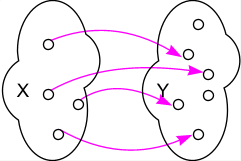
\includegraphics[scale=0.5]{injektiv.png}

\paragraph{Injektivität zeigen}
Injektiv wird meist direkt über die zweite Eigenschaft gemacht oder per Wiederspruchsbeweis (indirekter Beweis) mittels der ersten Eigenschaft bewiesen.
\todo{Beispiel?}

\paragraph{Eigenschaften}
\begin{itemize}
	\item Die Gleichung $f(x) = y$, $f$ ist injektiv und $y$ gegeben, verfügt über eine oder keine Lösung für $x$
	\item Eine \textit{stetige reelwertige} Funktion auf einem \textit{reelen Intervall} ist genau dann \underline{injektiv}, wenn sie in ihrem gesamten Definitionsbereich \textit{streng monoton} steigend oder fallend ist.
	\item Sind die beiden Funktionen $g, f$ injektiv, so ist die \underline{Komposition} $g \circ f$ ebenfalls injektiv
	\item Ist $g \circ f$ injektiv, so ist $f$ injektiv
	\item $f: M \rightarrow N$ ist injektiv, wenn es die \underline{links inverse} Funktion $g: N \rightarrow M$ gibt, so dass $g \circ f = \id_M$
\end{itemize}

\subsubsection{Surjektiv}
Sei $f: M \rightarrow N$, $f$ ist surjektiv, wenn folgendes gilt:
\begin{align*}
\forall y \in N: \exists x \in M: f(x) = y
\end{align*}
Wenn also für jedes Element aus $N$ mindestens ein (können auch mehr sein) Element in $M$ gibt, dass auf das Element aus $N$ zeigt.

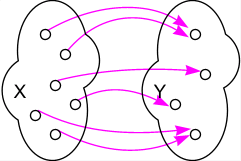
\includegraphics[scale=0.5]{surjektiv.png}

\paragraph{Eigenschaften}
\begin{itemize}
	\item Die Gleichung $f(x) = y$, $f$ ist surjektiv und $y$ gegeben, verfügt über eine oder mehrere Lösungen für $x$.
	\item Sind die Funktionen $f: A \rightarrow B$ und $g: B \rightarrow C$ surjektiv, so ist die \underline{Komposition} $g \circ f: A \rightarrow C$ auch surjektiv
	\item Ist $g \circ f$ surjektiv, so folgt, dass $g$ surjektiv ist
	\item $f: A \rightarrow B$ ist genau dann surjektiv, wenn $f$ ein \underline{rechtes Inverse} hat, also $g: B \rightarrow A$ mit $f \circ g = \id_B$
\end{itemize}

\subsubsection{Bijektiv}
Eine Funktion ist bijektiv, wenn sie injektiv und surjektiv ist.

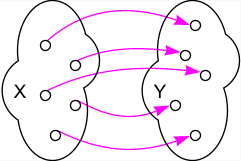
\includegraphics[scale=0.5]{bijektiv.png}

\paragraph{Eigenschaften}
\begin{itemize}
	\item Es gelten die Eigenschaften von Injektivität und Surjektivität
	\item Die Gleichung $f(x) = y$, $f$ ist bijektiv und $y$ gegeben, verfügt über genau eine Lösung für $x$
	\item Sind die Funktionen $f: A \rightarrow B$ und $g: B \rightarrow C$ bijektiv, dann ist auch die \underline{Komposition} $g \circ f: A \rightarrow C$ bijektiv.
	\item Ist $g \circ f$ bijektiv, dann ist $f$ injektiv und $g$ surjektiv
\end{itemize}

\section{Folgen in $\R$}

\subsection{Definitionen}
\begin{description}
  \item[konvergent] $\lim_{x \to \infty} a_n$ existiert \index{konvergent}
  \item[divergent] $\lim_{x \to \infty} a_n$ existiert nicht \index{divergent}
  \item[Nullfolge] $\lim_{x \to \infty} a_n = 0$ gilt \index{Nullfolge}
  \item[beschränkt] Es gibt $C_1, C_2$, so dass gilt $C_1 \leq a_n \leq C_2$
  bzw. $C$ gibt, so dass $|a_n| \leq C$
  \item[unbeschränkt] falls $(a_n)$ nicht beschränkt ist. Unbeschränkte folgen
  sind stets \underline{divergent}
  \item[monoton wachsend] $a_n \leq a_{n+1} \quad \forall n \in \N$ \index{monoton}
  \item[streng monoton wachsend] $a_n < a_{n+1} \quad \forall n \in \N$
  \item[monoton fallend] $a_n \geq a_{n+1} \quad \forall n \in \N$
  \item[streng monoton fallend] $a_n > a_{n+1} \quad \forall n \in \N$
  \item[alternierend] die Vorzeichen der Folgenglieder wechseln sich ab
  \item[bestimmt divergent / uneigentlich konvergent] es gilt $\lim_{n \to
  \infty} a_n = \pm \infty$
\end{description}

\begin{definition}[Grenzwert] \index{Grenzwert}
	\begin{align*}
		\lim_{n \to \infty} a_n = a & \Leftrightarrow a_n \to a \\
		& \Leftrightarrow \forall \epsilon > 0 \exists n_0 \in \N \forall n \geq n_0:
		|a_n - a| < \epsilon
	\end{align*}
\end{definition}

\begin{definition}[Teilfolge] \index{Teilfolge}
Werden von einer Folge beliebig viele Glieder weggelassen, aber nur so viele,
dass noch unendlich viele übrigbleiben, so erhält man eine Teilfolge.
\end{definition}

\begin{definition}[Häufungspunkt] \index{Häufungspunkt}
	$a$ ist Häufungspunkt der Folge $(a_n)$, wenn in jeder Umgebung von $a$
	unendlich viele Folgeglieder liegen. Das ist äquivalent damit, dass $a$ der
	Limes einer Teilfolge von $(a_n)$ ist.
\end{definition}

\begin{definition}[Limes superior / Limes inferior] \index{$\limsup$}\index{$\liminf$}
	Ist $(a_n)$ eine beschränkte Folge, so heisst der grösste Häufungspunkt Limes
	superior ($\limsup_{n \to \infty} a_n$ oder $\overline{\lim}_{n \to \infty}
	a_n$). Der kleinste Häufungspunkt ist der Limes inferior ($\liminf_{n \to
	\infty} a_n$ oder $\underline{\lim}_{n \to \infty} a_n$)
\end{definition}

\subsection{Rechnen mit Eigenschaften}
Addition:
\begin{itemize}
  \item $(a_n), (b_n)$ konvergiert $\Rightarrow (a_n + b_n)$ konvergiert
  \item $(a_n)$ konvergiert, $(b_n)$ divergent $\Rightarrow (a_n + b_n)$
  divergent
  \item $(a_n)$ beschränkt, $(b_n)$ beschränkt $\Rightarrow (a_n + b_n)$
  beschränkt
  \item $(a_n)$ beschränkt, $(b_n)$ unbeschränkt $\Rightarrow (a_n + b_n)$
  unbeschränkt
  \item $(a_n)$ beschränkt, $(b_n) \to \pm \infty \Rightarrow (a_n + b_n) \to
  \pm \infty$
  \item $(a_n) \to \infty$, $(b_n) \to \infty \Rightarrow (a_n + b_n) \to \infty$
  \item $(a_n) \to -\infty$, $(b_n) \to -\infty \Rightarrow (a_n + b_n) \to
  -\infty$
\end{itemize}

Produkt:
\begin{itemize}
  \item $(a_n)$ Nullfolge, $(b_n)$ beschränkt $\Rightarrow (a_n b_n)$ Nullfolge
  \item $(a_n)$ konvergent, $(b_n)$ beschränkt $\Rightarrow (a_n b_n)$
  beschränkt
  \item $(a_n)$ konvergent, $(b_n)$ konvergent $\Rightarrow (a_n b_n)$
  konvergent
  \item $(a_n)$ konvergent gegen $a \neq 0$, $(b_n)$ divergent $\Rightarrow
  (a_n b_n)$ divergent
\end{itemize}

\subsection{Rechnen mit Grenzwerten}
$\lim_{n \to \infty} a_n = a$, $\lim_{n \to \infty} b_n = b$\\
\emph{\underline{Achtung!} Untenstehendes gilt \underline{nur} wenn die Grenzwerte von $a_n$ und $b_n$ existieren. (Nicht $0$ oder $\inf$ sind.)}
\begin{itemize}
  \item $\lim_{n \to \infty} (a_n \pm b_n) = a \pm b$
  \item $\lim_{n \to \infty} (c \cdot a_n) = c \cdot a$
  \item $\lim_{n \to \infty} (a_n b_n) = ab$
  \item \underline{Achtung:} $\lim_{n \to \infty} (a_n)^c = (\lim_{n \to
  \infty} a_n)^c$, nur wenn $c \neq n$
  \item $\lim_{n \to \infty} \frac{a_n}{b_n} = \frac{a}{b}, \quad (b_n)$ keine
  Nullfolge
\end{itemize}

\subsection{Hilfsmittel}
\textbf{Bernoullische Ungleichung}: Für $x \geq -1$ und $n \in \N$
\[
	(1+x)^n \geq 1 + nx
\]


\textbf{Vergleich von Folgen}: weiter rechts stehende Werte gehen schneller nach
$\infty$
\[
	1, \quad \ln n, \quad n^\alpha \; (\alpha > 0), \quad q^n \; (q > 1), \quad n!,
	\quad n^n
\]

\textbf{Stirlingformel}:
\[
	n! \approx \sqrt{2 \pi n} \left (\frac{n}{e} \right )^n
	\Rightarrow \left ( \frac{n}{e} \right )^n \sqrt{2 \pi n} \leq n! \leq \left (
	\frac{n}{e} \right )^n \sqrt{2 \pi n} \cdot e^\frac{12}{n}
\]

\subsection{Konvergenzkriterien}\index{Konvergenzkriterien}
\begin{align*}
	a_n \to a \Leftrightarrow a_n - a \to 0 \Leftrightarrow |a_n - a| \to 0
\end{align*}
	
\begin{itemize}[leftmargin=*]	
	\item Ist $\lim_{n \to \infty} a_n = a$, so ist der Limes $a$ einziger
	Häufungspunkt der Folge $(a_n)$ und jede Teilfolge konvergiert auch gegen $a$.
	
	\textbf{Beispiel:} Wegen $\left( 1 + \frac{1}{n} \right)^n \to e$, so gilt auch
	$\left( 1 + \frac{1}{2n} \right)^{2n} \to e$
	
	\item Hat die Folge zwei verschiedene Häufungspunkte, so ist die Folge sicher
	divergent.
	
	\item Ist die Folge monoton steigend und nach oben beschränkt, dann existiert
	$\lim_{n \to \infty} a_n$. Ist die Folge monoton fallend und nach unten
	beschränkt, dann existiert $\lim_{n \to \infty} a_n$
	
	\item Konvergiert $\sum_{n=0}^\infty a_n$, so ist $\lim_{n \to \infty} a_n =
	0$\\
	Damit kann die Regeln für Reihen verwenden. Siehe Grenzwerte von Reihen.
	
	\item Gibt es eine Funktion $f$ mit $f(n) = a_n$ und $\lim_{x \to \infty} f(x)
	= a$, so gilt auch $\lim_{n \to \infty} a_n = a$.\\
	Damit kann man zum Beispiel die Regel von \underline{l'Hospital} und die
	restlichen Methoden anwenden. Siehe Grenzwerte von Funktionen.\\
	\underline{Achtung:} Es kann sein, dass $f$ keinen Grenzwert besitzt, aber
	$(a_n)$ schon.
	
	\item \textbf{Einschliessungskriterium}: Sind $(a_n), (b_n), (c_n)$ Folgen mit
	$a_n \leq b_n \leq c_n$ und haben $(a_n), (c_n)$ den gleichen Grenzwert $a$, so
	konvergiert auch $(b_n)$ nach $a$.
\end{itemize}

\subsection{Tipps \& Beispiele}
\subsubsection{Brüche}
$\lim_{n \to \infty} \frac{n^2 + \ln n}{\sqrt{n^4 - n^3}}$

Bei Brüchen empfiehlt es sich den am stärksten wachsenden Teil (das am
schnellsten wachsende $n$) zu kürzen. In diesem Fall ist es das $n^4$ in der
Wurzel, also $n^2$.

\begin{align*}
\ldots &= \lim_{n \to \infty} \frac{n^2 + \ln n}{\sqrt{n^4 - n^3}}
\cdot \frac{\frac{1}{n^2}}{\frac{1}{n^2}} = \lim_{n \to \infty} \frac{n^2 + \ln
n}{n^2 \sqrt{1 - \frac{1}{n}}} \cdot \frac{\frac{1}{n^2}}{\frac{1}{n^2}} \\
&= \lim_{n \to \infty} \frac{1 + \frac{\ln n}{n^2}}{\sqrt{1 - \frac{1}{n}}}
= \frac{1 + 0}{\sqrt{1 - 0}} = 0
\end{align*}

\subsubsection{l'Hospital für Folgen (Folge als Funktion)}
$\lim_{n \to \infty} \frac{\ln n}{n^2}$

Die Funktion $f(x) = \frac{\ln x}{x^2}$ entspricht unseren Folgegliedern ($f(n)
= a_n = \frac{\ln n}{n^2}$). Für $n \to \infty$ hat der Nenner und der Zähler
den Grenzwert $\infty$, also wenden wir die Regel von l'Hospital an.

\begin{align*}
\ldots &= \lim_{x \to \infty} \frac{(\ln x)'}{(x^2)'} = \lim_{x \to \infty}
\frac{\frac{1}{x}}{2x} = \lim_{x \to \infty} \frac{1}{x^2} = 0
\end{align*}

Somit geht auch die Folge gegen 0.

\subsubsection{Wurzeln}
$\lim_{n \to \infty} (\sqrt{n^2 + an + 1} - \sqrt{n^2 + 1})$

Hier wendet man die dritte binomische Formel an, um den grenzwert zu berechnen.
Die einzelnen Terme streben jeweils gegen $\infty$ und $\infty - \infty$ kann
nicht berechnet werden.

\underline{Achtung} auf die Vorzeichen beim Anwenden der Regel!

\begin{align*}
&= \lim_{n \to \infty} (\sqrt{n^2 + an + 1} - \sqrt{n^2 + 1}) \cdot
\left(\frac{\sqrt{n^2 + an + 1} + \sqrt{n^2 + 1}}{\sqrt{n^2 + an + 1} +
\sqrt{n^2 + 1}} \right) \\
&= \lim_{n \to \infty} \frac{(n^2 + an + 1) - (n^2 + 1)}{\sqrt{n^2 + an + 1} +
\sqrt{n^2 + 1}} \\
&= \lim_{n \to \infty} \frac{an}{\sqrt{n^2 + an + 1} + \sqrt{n^2 + 1}} 
\end{align*}

nun verwenden wir den Tipp für Brüche und kürzen das $n$ heraus

\begin{align*}
\ldots &= \lim_{n \to \infty} \frac{a}{\sqrt{1 + \frac{a}{n} + \frac{1}{n^2}} +
\sqrt{1 + \frac{1}{n^2}}} = \frac{a}{1 + 1} = \frac{a}{2}
\end{align*}

\subsubsection{Laufvariable im Exponent}
$\lim_{x \to 0} (3 - |x|)^{\frac{\sin(x)}{x}}$\newline
$\Rightarrow (3 - |x|)^{\frac{\sin(x)}{x}} = e^{\frac{\sin(x)}{x} \cdot \ln(3 -
|x|)}$\newline
$\Rightarrow 
\lim_{x \to 0} (3 - |x|)^{\frac{\sin(x)}{x}} = \lim_{x \to 0}e^{\frac{\sin(x)}{x} \cdot \ln(3 -
|x|)}$\newline
$\Rightarrow \lim_{x \to 0}\frac{\sin(x)}{x}\cdot \ln(3-|x|) = \ln(3)$\newline
$\Rightarrow \lim_{x \to 0}(3 - |x|)^{\frac{\sin(x)}{x}} = e^{\ln(3)} = 3$


\subsubsection{Gruppieren}
%Aus Analysis II (2012) Serie 1 Aufgabe 2b
Hat man zum Beispiel die Folge $s_n = 1 + \frac{1}{3} + \frac{1}{5} + ... + \frac{1}{2n-1}$ so kann man die 
einzelnen Therme gruppieren und abschätzen in diesem Fall z.B. mit $\frac{1}{4}$ (zweiter Therm, dritter und vierter Therm,
fünfter bis achter Therm, nächste 8 Therme, etc.). Wir erhalten dann $s_{2^k} \geq 1 + \frac{k}{4}$ und sehen somit das die 
Reihe nicht beschränkt ist und somit auch nicht konvergiert.

\subsection{Cauchy-Folgen}\index{Cauchy-Folge}
\begin{definition}[Cauchy-Folge]
Sei $(a_n)_{n \in \N}$ eine Folge in $\R$. $(a_n)_{n \in \N}$ heisst \textbf{Cauchy-Folge}, falls gilt
\begin{align*}
\forall \epsilon > 0 \; \exists n_n = n_0(\epsilon) \in \N \; \forall n, l \geq n_0: |a_n - a_l| < \epsilon
\end{align*}
\end{definition}

Die Definition sagt grundsätzlich aus, dass ab einem $n_0(\epsilon)$ (also einem Anfang $n_0$, der abhängig von $\epsilon$ ist)
die Folgeglieder nur noch $\epsilon$ Abstand zu einander haben. Also der Abstand beliebig klein wird zwischen Folgegliedern.

\begin{satz}[Cauchy-Kriterium]
Für $(a_n)_{n \in \N} \subset \R$ sind äquivalent:
\begin{itemize}
	\item $(a_n)_{n \in \N}$ ist konvergent
	\item $(a_n)_{n \in \N}$ ist Cauchy-Folge
\end{itemize}
\end{satz}

\section{Reihen}

\subsection{Definitionen}
Eine Reihe $\sum_{n = 1}^\infty a_n$ ist \underline{konvergent} mit Grenzwert
$s$, wenn die Folge der \underline{Partialsummen} $(S_m)$, $S_m :=
\sum_{n=1}^m a_n$ gegen $s$ konvergiert. Also wenn gilt: $S_m \to s$.

\begin{definition}[$\epsilon$-Kriterium]
	$\forall \epsilon > 0 \; \exists n_0 \in \N \; \forall m \geq n_0: \left|
	\sum_{n=1}^m a_n - s \right| < \epsilon$
\end{definition}

\begin{definition}[Absolute Konvergenz]\index{Konvergenz}
Wenn auch die Reihe der Absolutbeträge $\sum_{n=1}^\infty |a_n|$ konvergiert, so
heisst die Reihe absolut konvergent. Aus der absoluten Konvergenz folgt
Konvergenz. Der Umkehrschluss ist nicht möglich.
\end{definition}

\subsection{Rechenregeln Reihen}
Für \underline{konvergente} Reihen gilt:
\[
	\sum_{n=1}^\infty a_n = A, \sum_{n=1}^\infty b_n = B \Rightarrow
	\sum_{n=1}^\infty (\alpha a_n + \beta b_n) = \alpha A + \beta B
\]

\subsection{Konvergenzkriterien}
\begin{tabular}{|l|}
\hline
	Konvergiert $\sum_{n=1}^\infty a_n$, so ist $\lim_{n \to \infty} a_n = 0$.\\
	Wenn also $\lim_{n \to \infty} a_n \neq 0$, so konvergiert die Reihe
	\underline{nicht}\\
\hline
\end{tabular}

\onecolumn

{\footnotesize
\begin{tabular}{|p{2cm}||p{3cm}|p{3cm}|p{3cm}|p{3cm}|p{3cm}|}
\hline & \multicolumn{4}{l}{schnelles Fallen} & langsames Fallen \\
\hline
 
wie schnell gehen die $a_n$ gegen 0 & exponentiell wie $q^n, |q| < 1$ &
polynominal wie $n^{-\alpha}, \alpha > 1$ & \multicolumn{2}{|c|}{höchstens wie
$1/n$} & gar nicht \\ \hline

Beispiele & \begin{align*} a_n = \frac{n^8}{2^n},\\ a_n =
(\sqrt[n]{n} - 1)^n,\\
a_n = \frac{1}{n!},\\ a_n = \left( \frac{-1}{4}\right)^n \end{align*} &
\begin{align*} a_n = \frac{1}{n^2}, \\ a_n = \frac{1}{n^{100}}, \\ a_n =
\frac{1}{(n + \ln n)^2}, \\ a_n = \frac{20}{n^2 - 33} \end{align*} &
\begin{align*} a_n = \frac{(-1)^n}{\ln n}, \\ a_n = \frac{(-1)^n}{n}
\end{align*} & \begin{align*} a_n = \frac{1}{\ln n}, \\ a_n = \frac{1}{n + \ln
n}, \\ a_n = \frac{1}{n} \end{align*} & \begin{align*} a_n = (-1)^n, \\ a_n =
\sin n, \\ a_n = n^2 \end{align*}\\ \hline

passende Konvergenzkriterien & Wurzel- und Quotientenkriterium & Integral- und
Verdichtungskriterium & Leibniz-Kriterium & & $a_n \not\to 0$ \\ \hline

Vergleichs-, Majoranten-, Minorantenkriterium & Vergleichen mit $q^n$ &
Vergleichen mit $n^{-\alpha}$ & kein Vergleich möglich & Vergleichen mit
$\frac{1}{n}$ & \\ \hline

Konvergenz-verhalten & \multicolumn{2}{c|}{absolute Konvergenz} & keine
absolute Konvergenz (einfach Konvergenz) & \multicolumn{2}{|c|}{Divergenz} \\
\hline

\end{tabular}
}

\begin{tabular}{|p{4cm}|p{15cm}|}\hline
\multicolumn{2}{|c|}{direkte Kriterien}\\ \hline

\textbf{Quotientenkriterium} & Gut für Reihen, die Fakultäten oder Glieder der
Form $a^n$ enthalten. Nicht auf Reihen anwendbar, in denen die Glieder nur wie
eine Potenz von $n$ fallen. \\ \hline

\textbf{Wurzelkriterium} & Gut in Reihen, deren Glieder $n$-te Potenzen sind,
zusammen mit der Stirlingformel oft auch bei Fakultäten anwendbar. \\ \hline

\textbf{Leibnizkriterium} & Nur für alternierende Reihen.\\ \hline

\textbf{Integralkriterium} & Anwendbar auf monotone Reihen.\\ \hline

\multicolumn{2}{|c|}{direkte Kriterien}\\ \hline

\textbf{Vergleichskriterium} & Ermöglicht es "`Störterme"' wegzulassen und so
einfachere Reihen zu untersuchen \\ \hline

\textbf{Verdichtungskriterium} & Bei monotonen Reihen anwendbar. Für Reihen mit
langsam fallenden Gliedern \\ \hline

\textbf{Majoranten- und Minorantenkriterium} & Ähnlich wie Vergleichskriterium.
Wird mit einer Reihe verglichen, deren Glieder stets kleiner oder grösser sind.
\\ \hline
\end{tabular}

\twocolumn

\subsubsection{Reihen Kriterien}
Achtung. Die nachfolgenden Kriterien sagen nur aus, ob die Reihen konvergiert
oder nicht. Sie sagen \underline{nicht} aus, gegen was sie konvergieren!

\paragraph{Quotientenkriterium}
\[
\left| \frac{a_{n+1}}{a_n} \right| \to q. \quad \text{Dann gilt} \begin{cases}
q < 1 & \Rightarrow \sum_{n=1}^\infty a_n \text{ konvergiert absolut} \\
q = 1 & \Rightarrow \text{keine Aussage}\\
q > 1 & \Rightarrow \sum_{n=1}^\infty a_n \text{ divergiert}
\end{cases}
\]

\paragraph{Wurzelkriterium}
\[
\sqrt[n]{\left | a_n \right |} \to q. \quad \text{Dann gilt} \begin{cases}
q < 1 & \Rightarrow \sum_{n=1}^\infty a_n \text{ konvergiert absolut}\\
q = 1 & \Rightarrow \text{keine Aussage}\\
q > 1 & \Rightarrow \sum_{n=1}^\infty a_n \text{ divergiert}
\end{cases}
\]

\paragraph{Leibnizkriterium}
Wenn gilt:
\begin{itemize}
  \item $(a_n)$ ist alternierende Folge, d.h die Vorzeichen wechseln jedes Mal
  \item $a_n \to 0$ oder $|a_n| \to 0$
  \item $(|a_n|)$ ist monoton fallend
\end{itemize}
\ldots dann konvergiert $\sum_{n=1}^\infty a_n$

\paragraph{Majorantenkriterium}
Ist $|a_n| \leq b_n$ und $\sum_{n=1}^\infty b_n$ konvergent, so konvergiert
$\sum_{n=1}^\infty a_n$ absolut.

\paragraph{Minorantenkriterium}
Ist $a_n \geq b_n \geq 0$ und $\sum_{n=1}^\infty b_n$ divergent, so divergiert
$\sum_{n=1}^\infty a_n$

\subsection{Potenzreihe}
Die Potenzreihe hat die allgemeine Form
\[
\sum_{n=0}^\infty a_n (x - x_0)^n
\]

$x_0$ ist der Entwicklungspunkt der Potenzreihe und $(a_n)_{n \in \N}$ eine
beliebige Folge.

\subsubsection{Konvergenzradius}
Die Berechnung des Konvergenzradius ist für solche Reihen einfacher, da der
Faktor $(x - x_0)$ nicht analysiert werden muss. Entsprechend gilt für den
Konvergenzradius $r$:
$r = \frac{1}{\limsup_{n\to\infty} \sqrt[n]{\|a_n\|}}$ (Wurzelkriterium) bzw.
$r = \lim_{n\to\infty} \left | \frac{a_n}{a_{n+1}} \right |$
(Quotientenkriterium).


\clearpage
\section{Formeltafel}
\subsection{Mitternachtsformel}
\[ a x + b x + c = 0 \qquad \implies \qquad x_{1,2} = \frac{-b \pm \sqrt{b^2-4ac}}{2a} \]

\subsection{Binomialkoeffizient}
\[ \binom nk = \frac{n!}{k!\,(n-k)!} \quad \mbox{für }\ 0\leq k\leq n \]

\subsection{Argument}
\[
	\arg(x,y) := \begin{cases}
		\arctan(\frac{y}{x}) & x \geq 0 \\
		-\arctan(\frac{y}{x}) & x < 0 \\
		\frac{\pi}{2} & x=0, y < 0 \\
		\frac{3\pi}{2} & x = 0, y > 0
	\end{cases}
\]

\subsection{Kreisfunktionen}
{\footnotesize
\begin{tabular}{|l||c|c|c|c|c|c|c||c|c|}\hline
\multirow{2}{*}{$\alpha$} & $0$ & $\frac{\pi}{6}$ & $\frac{\pi}{4}$ &
$\frac{\pi}{3}$ & $\frac{\pi}{2}$ & $\frac{2\pi}{3}$ & $\pi$ &
\multirow{2}{*}{Periode} & \multirow{2}{*}{Wertebereich}\\

& $0^\circ$ & $30^\circ$ & $45^\circ$ & $60^\circ$ & $90^\circ$ & $120^\circ$ &
$180^\circ$ & &\\ \hline

$\sin$ & $0$ & $\frac{1}{2}$ & $\frac{\sqrt{2}}{2}$ &
$\frac{\sqrt{3}}{2}$ & $1$ & $\frac{\sqrt{3}}{2}$ & $0$ & $\sin(\alpha +
k\cdot$\hl{$2\pi$}$)$ & $[-1,1]$\\ \hline

$\cos$ & $1$ & $\frac{\sqrt{3}}{2}$ & $\frac{\sqrt{2}}{2}$ & $\frac{1}{2}$ & $0$
& $-\frac{1}{2}$ & $-1$ & $\cos(\alpha + k\cdot$\hl{$2\pi$}$)$ & $[-1,1]$\\
\hline


$\tan$ & $0$ & $\frac{\sqrt{3}}{3}$ & $1$ & $\sqrt{3}$ & $\pm \infty$ &
$-\sqrt{3}$ & $0$ & $\tan(\alpha + k \cdot$\hl{$\pi$}$)$ & $]-\infty, \infty[$
\\
\hline
\end{tabular}
}
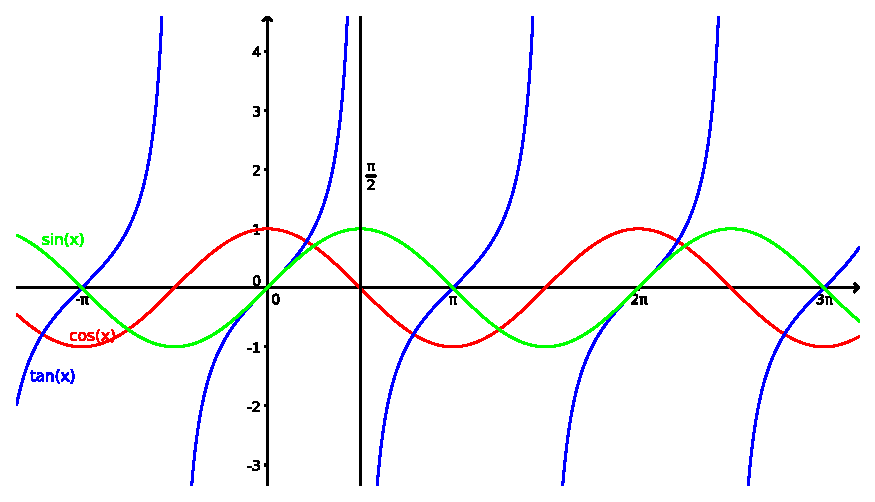
\includegraphics[width=\columnwidth]{sin_cos_tan.eps}

\subsubsection{Einheitskreis}
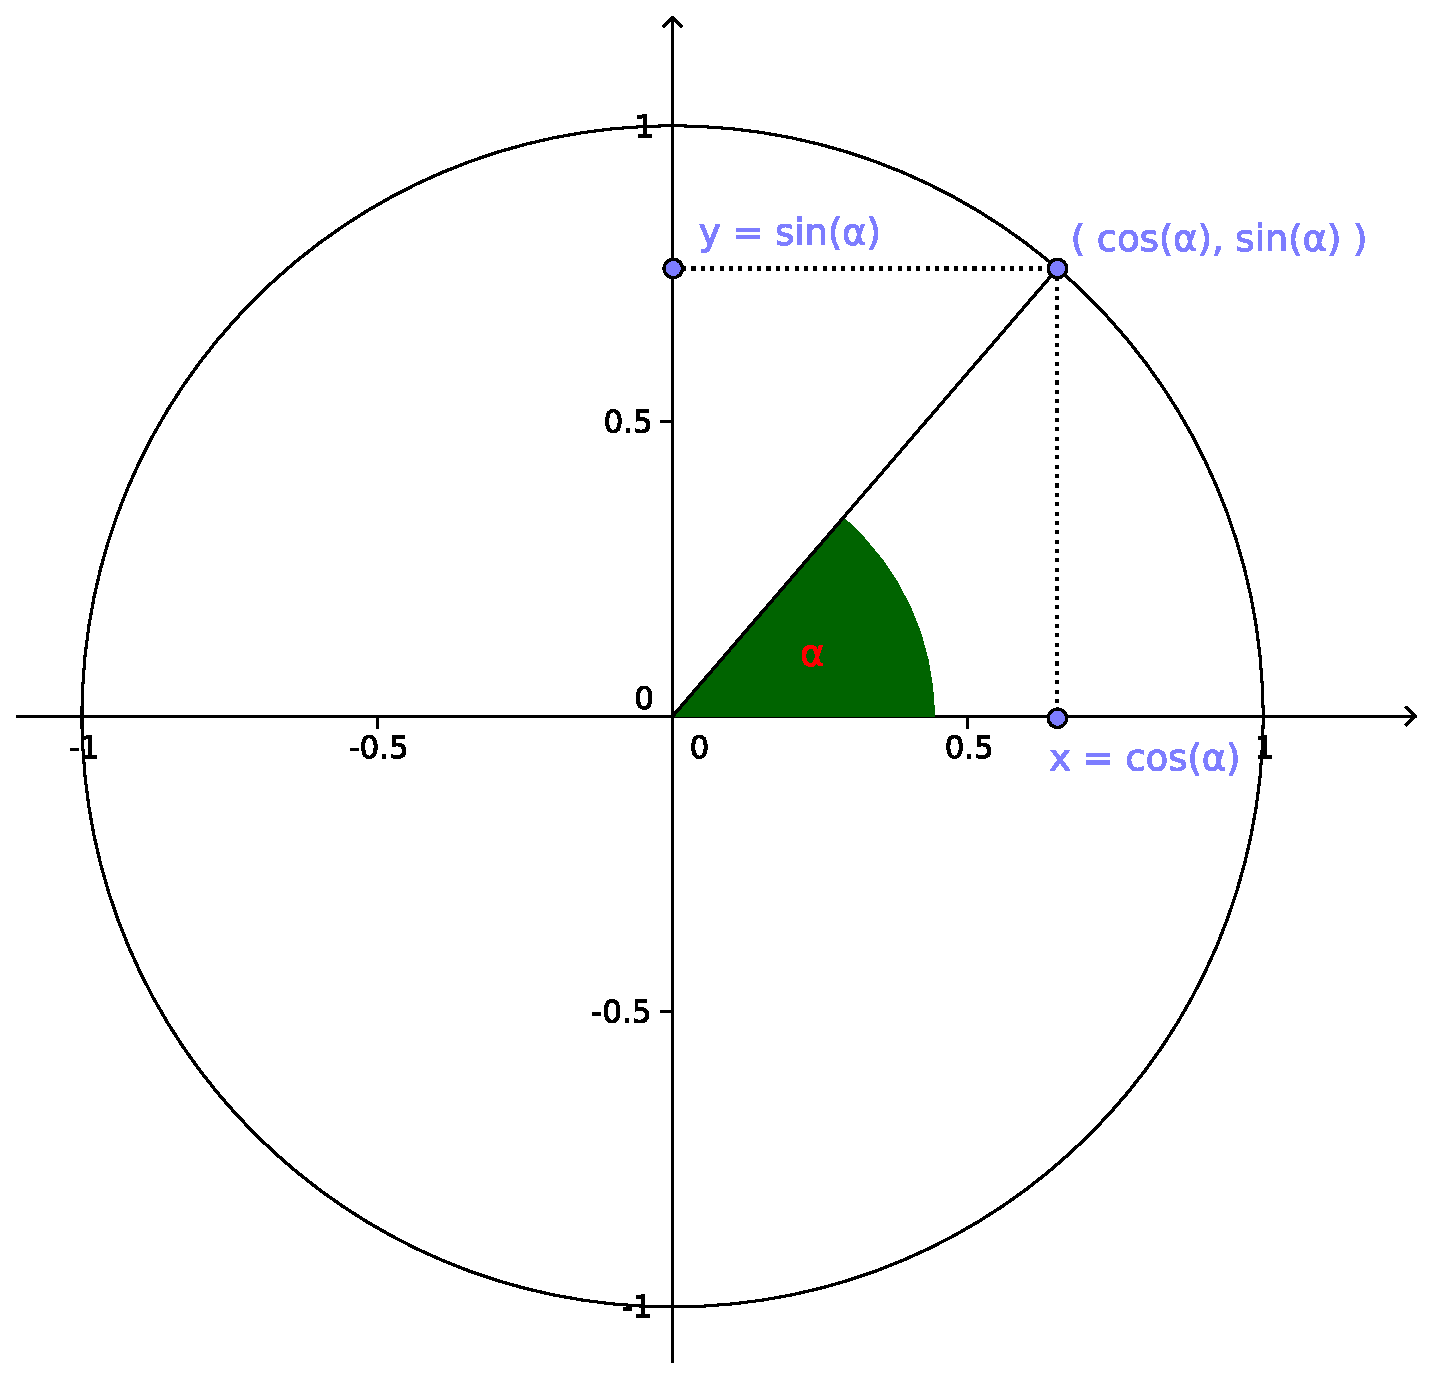
\includegraphics[width=\columnwidth]{einheitskreis_sin_cos.eps}
$\tan \alpha = \frac{\sin \alpha}{\cos \alpha} = \frac{y}{x}$

\subsection{Trigonometrische Funktionen \& Additionstheorem}
\begin{itemize}[leftmargin=*]
	\item $\sin^2(x) + \cos^2(x) = 1$
	\item $\frac{1}{\cos^2(\alpha)} = 1 + \tan^2(\alpha)$
	\item $\sin(90^\circ \pm \alpha) = \cos(\alpha)$
	\item $\sin(180^\circ \pm \alpha) = \mp \sin(\alpha)$
	\item $\cos(90^\circ \pm \alpha) = \mp \sin(\alpha)$
	\item $\cos(180^\circ \pm \alpha) = - \cos(\alpha)$
	\item $\sin(\alpha \pm \beta) = \sin(\alpha)\cos(\beta) \pm
	\cos(\alpha)\sin(\beta)$
	\item $\cos(\alpha \pm \beta) = \cos(\alpha)\cos(\beta) \mp \sin(\alpha)
	\sin(\beta)$
	\item $\tan(\alpha \pm \beta) = \frac{\tan(\alpha) \pm \tan(\beta)}{1 \mp
	\tan(\alpha)\tan(\beta)}$
	\item $\sin(2\alpha) = 2 \sin(\alpha)\cos(\alpha)$
	\item $\cos(2\alpha) = \cos^2(\alpha) - \sin^2(\alpha) = 2 \cos^2(\alpha) - 1
	= 1 - 2 \sin^2(\alpha)$
	\item $\tan(2\alpha) = \frac{2 \tan(\alpha)}{1 - \tan^2(\alpha)}$
\end{itemize}

\subsection{Hyperbelfunktionen}
\begin{itemize}[leftmargin=*]
	\item $\sinh(x) = \frac{1}{2}(e^x - e^{-x}) = -i \sin(ix)$
	\item $\cosh(x) = \frac{1}{2}(e^x + e^{-x}) = \cos(ix)$
	\item $\tanh(x) = \frac{\sinh(x)}{\cosh(x)} = \frac{e^x - e^{-x}}{e^x +
	e^{-x}} = \frac{e^{2x} - 1}{e^{2x} + 1} = 1 - \frac{2}{e^{2x} + 1}$
	\item $\arcsinh(x) = \ln(x + \sqrt{x^2 + 1})$
	\item $\arcosh(x) = \ln(x + \sqrt{x^2 - 1})$
	\item $\arctanh(x) = \frac{1}{2} \ln(\frac{1+x}{1-x})$
	\item Umformung: $\tanh(x) + 1 = \frac{e^{2x} - 1}{e^{2x} + 1} + 1 = \frac{2x -
	1 + e^{2x} + 1}{e^{2x} + 1} = \frac{2e^{2x}}{e^{2x} + 1}$
\end{itemize}


\subsection{Ableitungen}
\subsection{Regeln}
\begin{itemize}[leftmargin=*]
	\item (Summenregel) $(f + g)'(x) = f'(x) + g'(x)$
	\item (Produktregel) $(fg)'(x) = f'(x)g(x) + f(x)g'(x)$
	\item (Quotientenregel) $(\frac{f}{g})'(x) = \frac{f'(x)g(x) -
	f(x)g'(x)}{g^2(x)}$
	\item (Kettenregel) $(g \circ f)'(x) = (g(f(x)))' = g'(f(x)) f'(x)$
\end{itemize}

\subsection{Ableitungs-Tafel}
\begin{itemize}[leftmargin=*]
	\item $\frac{d}{dx}\; x^n = nx^{n-1}$
	\item $\frac{d}{dx}\; \frac{1}{x^n} = -n \frac{1}{x^{n+1}}$
	\item $\frac{d}{dx}\; \sqrt[n]{x} = \frac{1}{n\sqrt[n]{x^{n-1}}}$
	\item $\frac{d}{dx}\; e^{\alpha x + \beta} = \alpha e^{\alpha x + \beta}$
	\item $\frac{d}{dx}\; \ln(x) = \frac{1}{x}$
	\item $\frac{d}{dx}\; \alpha^x = \alpha^x \ln(\alpha)$
	\item $\frac{d}{dx}\; x^x = x^x (1 + \ln(x))$
	\item $\frac{d}{dx}\; \sin(\alpha x + \beta) = \alpha \cos(\alpha x + \beta)$
	\item $\frac{d}{dx}\; \cos(\alpha x + \beta) = -\alpha \sin(\alpha x + \beta)$
	\item $\frac{d}{dx}\; \tan(\alpha x + \beta) = \alpha \frac{1}{\cos^2(\alpha x
	+ \beta)}$
	\item $\frac{d}{dx}\; \sinh(\alpha x + \beta) = \alpha \cosh(\alpha x + \beta)$
	\item $\frac{d}{dx}\; \cosh(\alpha x + \beta) = \alpha \sinh(\alpha x + \beta)$
	\item $\frac{d}{dx}\; \tanh(\alpha x + \beta) = \alpha
	\frac{1}{\cosh^2(\alpha x + \beta)}$
	\item $\frac{d}{dx}\; \arcsin(\alpha x + \beta) =
	\frac{\alpha}{\sqrt{1-(\alpha x + \beta)^2}}$;  
		$\frac{d}{dx}\; \arcsin(x) = \frac{1}{\sqrt{1-x^2}}$
	\item $\frac{d}{dx}\; \arccos(\alpha x + \beta) = -\frac{\alpha}{\sqrt{1 -
	(\alpha x + \beta)^2}}$;
		$\frac{d}{dx}\; \arccos(x) = -\frac{1}{\sqrt{1-x^2}}$
	\item $\frac{d}{dx}\; \arctan(\alpha x + \beta) = \frac{\alpha}{(\alpha x +
	\beta)^2 + 1}$; 
		$\frac{d}{dx}\; \arctan(x) = \frac{1}{x^2+1}$
	\item $\frac{d}{dx}\; x^{x^\alpha} = x^{x^\alpha + \alpha - 1} (\alpha
	\log(x) + 1)$
	\item $\frac{d}{dx}\; e^{x^\alpha} = \alpha x^{\alpha - 1} e^{x^\alpha}$
\end{itemize}

\subsection{Integrale}
\subsubsection{Integralregeln}
Es gelte: $\int f(x) \, dx = F(x)$
\begin{itemize}[leftmargin=*]
	\item $\int u'\cdot v dx = uv - \int u \cdot v' dx$
	\item $\int f(x) dx = \int f(g(t)) \cdot g'(t) dt, \; x=g(t), dx = g'(t) dt$\newline\hfill
	\item $\int f(a + x) \,dx = F(a + x)$
	\item $\int f(a - x) \,dx = -F(a-x)$
	\item $\int f(-x) \,dx = -F(-x)$
	\item $\int f(\alpha x) \,dx = \frac{1}{\alpha}F(\alpha x)$
	\item $\int \frac{g'(x)}{g(x)} \, dx = \ln|g(x)|$
	\item $\int g(x)g'(x) \, dx = \frac{1}{2}g(x)^2$
\end{itemize}
\subsubsection{typische Integrale}
\begin{itemize}[leftmargin=*]
  	\item $\int \frac{1}{x} \,dx = \ln |x|$
  	\item $\int \frac{1}{x+a} \,dx = \ln |x+a|$
  	\item $\int \ln(x) \,dx = x(\ln(x) - 1)$
  	\item $\int \ln(ax + b) \,dx = \frac{(a x+b) \ln (a x+b)-a x}{a}$
  	\item $\int \frac{1}{(x+a)^2} \,dx = - \frac{1}{x+a}$
  	\item $\int \frac{1}{\sqrt{x}} \,dx = 2 \sqrt{x}$
	\item $\int \frac{1}{ax+b} \,dx = \frac{1}{a} \ln |ax+b|$
	\item $\int(ax + b)^n \,dx = \frac{(ax + b)^{n+1}}{(n + 1)a}, (n \neq -1)$
	\item $\int x(ax+b)^n \,dx = \frac{(ax + b)^{n+2}}{(n+2)a^2} -
	\frac{b(ax+b)^{n+1}}{(n+1)a^2}$
	\item $\int \frac{ax + b}{px + q} \,dx = \frac{ax}{p} + \frac{bp - aq}{p^2} \ln
	|pq+q|$
	\item $\int \frac{1}{a^2 + x^2} \,dx = \frac{1}{a} \arctan(\frac{x}{a})$
	\item $\int \frac{1}{a^2 - x^2} \,dx = \frac{1}{2a} \ln \left | \frac{a+x}{a-x}
	\right |$
	\item $\int \sqrt{x} \,dx = \frac{2}{3}\sqrt{x^3}$
	\item $\int a^{xb + c} \,dx = \frac{a^{bx + c}}{b \log(a)}$
\end{itemize}

\subsubsection{trionometrische Funktionen}
\begin{itemize}[leftmargin=*]
	\item $\int \sin(ax) \,dx = -\frac{1}{a}\cos(ax)$
	\item $\int \cos(ax) \,dx = \frac{1}{a}\sin(ax)$
	\item $\int \sin(ax)^2 \,dx = \frac{x}{2} - \frac{sin(2ax)}{4a}$
	\item $\int \frac{1}{\sin^2 x} \,dx = -\cot x$
	\item $\int x \sin(ax) \,dx = \frac{\sin(ax)}{a^2} - \frac{x \cos(ax)}{a}$
	\item $\int \cos^2(ax) \,dx = \frac{x}{2} + \frac{\sin(2ax)}{4a}$
	\item $\int \frac{1}{\cos^2(x)} \,dx = \tan x$
	\item $\int \cos(ax) \,dx = \frac{\cos(ax)}{a^2} + \frac{x \sin(ax)}{a}$
	\item $\int \sin(ax) \cos(ax) \,dx = -\frac{\cos^2(ax)}{2a}$
	\item $\int \tan(ax) \,dx = - \frac{1}{a} \ln | \cos(ax) |$
	\item $\int \arcsin(x) \,dx = x \arcsin(x) + \sqrt{1 - x^2}$
	\item $\int \arccos(x) \,dx = x \arccos(x) - \sqrt(1-x^2)$
	\item $\int \arctan(x) \,dx = x \arctan(x) - \frac{1}{2} \ln(1+x^2)$
\end{itemize}

\subsubsection{Hyperbelfunktionen}
\begin{itemize}[leftmargin=*]
	\item $\int \sinh(ax + b) \,dx = \frac{\cosh(ax + b)}{a}$; $\int \sinh(x) \,dx
	= \cosh(x)$
	\item $\int \cosh(ax + b) \,dx = \frac{\sinh(ax + b)}{a}$; $\int \cosh(x) \,dx
	= \sinh(x)$
	\item $\int \tan(ax + b) \,dx = \frac{\log(\cosh(ax+b))}{a}$; $\int \tan(x)
	\,dx = \log(\cosh(x))$
\end{itemize}

\subsubsection{Exponentialfunktion}
\begin{itemize}[leftmargin=*]
  	\item $\int e^{ax} \,dx = \frac{1}{a} e^{ax}$ 
	\item $\int x e^{ax} \,dx = e^{ax} \cdot \left ( \frac{ax - 1}{a^2} \right )$
	\item $\int x \ln(x) \,dx = \frac{1}{2} x^2 (\ln(x) - \frac{1}{2})$
	\item $\int_{-\infty}^\infty e^{-\frac{1}{a}x^2} \,dx = \sqrt{a \pi}$
\end{itemize}

\subsection{Reihenentwicklung}
\begin{itemize}[leftmargin=*]
	\item $e^x = \sum_{n=0}^\infty \frac{x^n}{n!} = 1 + \frac{x}{1!} +
	\frac{x^2}{2!} + \cdots$
	\item $\sin x = \sum_{n=0}^\infty (-1)^n \frac{x^{2n + 1}}{(2n + 1)!} = x -
	\frac{x^3}{3!} + \frac{x^2}{5!} + \cdots$
	\item $\cos x = \sum_{n=0}^\infty (-1)^n \frac{x^{2n}}{(2n)!} = 1 -
	\frac{x^2}{2!} + \frac{x^4}{4!} - \cdots + \cdots$
	\item $\sinh x = \sum_{n=0}^\infty \frac{x^{2n+1}}{(2n + 1)!}$
	\item $\cosh x = \sum_{n=0}^\infty \frac{x^{2n}}{(2n)!}$
	\item $\ln x = \sum_{n=0}^\infty \frac{2}{2n + 1} \cdot \left(
	\frac{x-1}{x+1} \right)^{2n}$
\end{itemize}

\subsection{Grenzwerte}
\begin{itemize}[leftmargin=*]
	\item \textbf{Bernoullische Ungleichung}: $x \geq -1, n \in \N: \; (1+x)^n \geq
	1+nx$
	\item \textbf{Vergleich von Folgen}: weiter rechts stehende Folgen streben
	schneller gegen $\infty$ als die links davon stehenden: $1, \quad \ln n, \quad
	n^\alpha (\alpha > 0), \quad q^n (q > 1), \quad n!, \quad n^n$ $\Rightarrow
	\lim_{x \to \infty} \frac{\ln n}{n^\alpha} = 0$
\end{itemize}
\subsubsection{$\lim_{n \to \infty}$}
\begin{itemize}[leftmargin=*]
	\item $\lim_{n \to \infty} \sqrt[n]{a} \rightarrow 1$
	\item $\lim_{n \to \infty} \sqrt[n]{n} \rightarrow 1$
	\item $\lim_{n \to \infty} \sqrt[n]{n!} \rightarrow \infty$
	\item $\lim_{n \to \infty} \frac{n}{\sqrt[n]{n!}} \rightarrow e$
	\item $\lim_{n \to \infty} \frac{1}{n} \sqrt[n]{n!} \rightarrow \frac{1}{e}$
	\item $\lim_{n \to \infty} \left ( \frac{n+1}{n} \right )^n \rightarrow e$
	\item $\lim_{n \to \infty} \left ( 1 + \frac{1}{n} \right )^n \rightarrow e$
	\item $\lim_{n \to \infty} \left ( 1 - \frac{1}{n} \right )^n \rightarrow \frac{1}{e}$
	\item $\lim_{n \to \infty} \left ( 1 + \frac{x}{n} \right )^n \rightarrow e^x$
	\item $\lim_{n \to \infty} \left ( 1 - \frac{x}{n} \right )^n \rightarrow \frac{1}{e^x}$
	\item $\lim_{n \to \infty} {a \choose n} \rightarrow 0, \; a > -1$
	\item $\lim_{n \to \infty} \frac{a^n}{n!} \rightarrow 0$
	\item $\lim_{n \to \infty} \frac{n^n}{n!} \rightarrow \infty$
	\item $\lim_{n \to \infty} \frac{a^n}{n^k} \rightarrow \infty, a > 1, k$ fest
	\item $\lim_{n \to \infty} a^n n^k \rightarrow 0, |a| < 1, k$ fest
	\item $\lim_{n \to \infty} n(\sqrt[n]{a} - 1) \rightarrow \ln a, a > 0$
	\item $\lim_{n \to \infty} \left( 1+\frac{x}{n} \right)^n = e^x \quad$
	\item $\lim_{n \to \infty} \sqrt[n]{n} = 1$
	\item $\lim_{n \to \infty} n^p q^n = 0 \qquad p \in \N \text{ und } 0 < q < 1$
	\item $\lim_{x \to \infty} \sqrt{x^2-x}-x = \frac{1}{2}$ \newline{\small (Lösungsansatz mit Taylorreihe
	($\sqrt{1-x} = 1 + \frac{x}{2}+O(x^2)$): $\sqrt{x^2-x}-x = x(\sqrt{1-\frac{1}{x}}-1) =
	x((1+\frac{1}{2x}+O(\frac{1}{x^2}))-1) = \frac{1}{2}+O(\frac{1}{x}) \underset{n \to \infty}{\longrightarrow} \frac{1}{2}$ )}
\end{itemize}
\subsubsection{$\lim_{x \to 0}$}
\begin{itemize}[leftmargin=*]
	\item $\lim_{x \to 0} \frac{a^x - 1}{x} = \ln a$
	\item $\lim_{x \to 0} \frac{\sin x}{x} = 1$
	\item $\lim_{x \to 0} \frac{1 - \cos x}{x} = 0$
	\item $\lim_{x \to 0} \frac{\log_a (1 + x)}{x} = \frac{1}{\ln a}$
	\item $\lim_{x \to 0} x^a \ln x = 0, \; a  > 0$
	\item $\lim_{x \to 0} \frac{a^x-1}{x} = \ln a$ 
	\item $\lim_{x \to 0} \frac{\sin(x)}{x} = 1$ 
	\item $\lim_{x \to 0} \frac{1-\cos(x)}{x} = 0 \quad$ 
	\item $\lim_{x \to 0} \frac{\log_a(1+x)}{x} = \frac{1}{\ln a}$
	\item $\lim_{x \to 0} x^\alpha \ln x = 0 \qquad \alpha > 0$
\end{itemize}

\subsection{Reihen}
\begin{itemize}[leftmargin=*]
	\item $\sum_{n=1}^\infty \frac{1}{n}$ divergiert (``harmonische Reihe'')
	\item $\sum_{n=1}^\infty \frac{(-1)^n}{n} = \ln \frac{1}{2}$
	\item $\sum_{n=1}^\infty \frac{1}{n^\alpha}$ konvergiert für $\alpha > 1$,
	divergiert für $\alpha \leq 1$
	\item $\sum_{n=1}^m n = \frac{m(m+1)}{2}$
	\item $\sum_{n=0}^\infty q^n = \frac{1}{1-q}$ für $|q| < 1$ (``geometrische
	Reihe'')
	\item $\sum_{n=0}^\infty (-1)^n q^n = \frac{1}{1-q}$ für $|q| < 1$ (``geometrische
	Reihe'')
	\item $\sum_{n=1}^\infty \frac{1}{n^2} = \frac{\pi^2}{6}$
	\item $\sum_{n=0}^m q^n = \frac{1-q^{m+1}}{1-q}$ 
	% ist in einer serie vorgekommen:
	\item  $\sum_{n=0}^m n^2 = \frac{1}{6}m(m+1)(2m+1)$
	\item  $\sum_{n=0}^m n^3 = \frac{1}{4}m^2(m+1)^2$
\end{itemize}

\subsection{Kreuzprodukt}
{\footnotesize
\[
\vec{a} \times \vec{b} = \left ( \begin{array}{c} a_1 \\ a_2 \\ a_3 \end{array}
\right ) \times
\left ( \begin{array}{c} b_1 \\ b_2 \\ b_3 \end{array}
\right ) =
\left ( \begin{array}{c} a_2b_3 - a_3b_2 \\ a_3b_1 - a_1b_3 \\ a_1b_2 - a_2b_1
\end{array} \right )
\]
}

\begin{multicols}{2}
\subsection{Exponent}
\begin{itemize}[leftmargin=*]
  \item $a^n a^m = a^{n + m}$
  \item $(a^n)^m = a^{nm}$
  \item $(ab)^n = a^n b^n$
  \item $\left( \frac{a}{b} \right)^n = \frac{a^n}{b^n}$
  \item $a^{-n} = \frac{1}{a^n}$
  \item $\left( \frac{a}{b} \right)^{-n} = \left( \frac{b}{a} \right)^n$
  \item $a^\frac{n}{m} = (a^\frac{1}{m})^n = (a^n)^\frac{1}{m}$
\end{itemize}
\columnbreak

\subsection{Wurzel}
\begin{itemize}[leftmargin=*]
  \item $\sqrt[n]{a} = a^\frac{1}{n}$
  \item $\sqrt[n]{ab} = \sqrt[n]{a} \sqrt[n]{b}$
  \item $\sqrt[m]{\sqrt[n]{a}} = \sqrt[nm]{a}$
  \item $\sqrt[n]{\frac{a}{b}} = \frac{\sqrt[n]{a}}{\sqrt[n]{b}}$
\end{itemize}

\end{multicols}

\subsection{Ungleichungen}
\begin{itemize}[leftmargin=*]
  \item $a < b \Rightarrow a + c < b + c$ und $a - c < b - c$
  \item $a < b$ und $c > 0 \Rightarrow \frac{a}{c} < \frac{b}{c}$
  \item $a < b$ und $c < 0 \Rightarrow \frac{a}{c} > \frac{b}{c}$ 
  \item Dreiecksungleichung für reelle Zahlen: $|a+b| \le |a|{+}|b|$ %Quelle Wikipedia: http://de.wikipedia.org/wiki/Dreiecksungleichung#Dreiecksungleichung_f.C3.BCr_reelle_Zahlen
  \item Cauchy-Schwarz Ungleichung: $|x \cdot y| \leq \|x\| \cdot \|y\|, \; x,y \in \R^n$
\end{itemize}

\subsection{Logarithmen}
\begin{itemize}[leftmargin=*]
  \item $y = \log_a x \Leftrightarrow x = a^y$
  \item $\log_a 1 = 0$
  \item $\log_a a^x = x$
  \item $a^{\log_a x} = x $
  \item $\log_a xy = \log_a x + \log_a y$
  \item $\log_a \frac{1}{x} = - \log_a x$
  \item $\log_a x^r = r \log_a x$
  \item $\log_a x = \frac{\log_b x}{\log_b a}$
  \item $\log_a x = \frac{\ln x}{\ln a}$
  \item $\log_a (x+y) = \log_a x + log_a (1 + \frac{y}{x})$
  \item $\log_a (x-y) = \log_a x + \log_a (1- \frac{y}{x})$
\end{itemize}

\subsection{Komplexe Zahlen}
\begin{itemize}[leftmargin=*]
	\item $z \in \C: z = a + b\cdot i$
	\item $i^2 = -1$
	\item $(a + bi) + (c + di) = (a + c) + (b + d)i$
	\item $(a + bi) \cdot (c + di) = (ac - bd) + (ad + bc)i$
	\item $\frac{a + bi}{c + di} = \frac{ac + bd}{c^2 + d^2} + \frac{bc - ad}{c^2 + d^2}\cdot i$
\end{itemize}

\subsection{Geometrische Körper}
\subsubsection{Ellipsoid}
Hat die Form eines Rugbyballs. In kartesischen Koordinaten definert durch
$\frac{x^2}{a^2} + \frac{y^2}{b^2} + \frac{z^2}{c^2} - 1 = 0$.

\subsection{Ausklammern}
\begin{itemize}[leftmargin=*]
	\item $x^n - y^n = (x-y) (x^{n-1} + x^{n-2}y + x^{n-3}y^2 + \ldots + xy^{n-2}
	+ y^{n-1})$
	\item $x^n - 1 = (x-1)(x^{n-1} + x^{n-2} + \ldots + x + 1)$
\end{itemize}

\subsection{Aus Serien}
\begin{itemize}[leftmargin=*]
	\item Ableitung von $x^x$ kann man berechnen, indem man $x = e^{\log(x)}$
	setzt. Also in diesem Fall $e^{\log(x^x)} = e^{x \log(x)}$ ableitet, was $e^{x
	\log(x)} (1 + \log(x))$ (Serie 10)
	\item Cauchy-Schwarz Ungleichung: $|x \cdot y| \leq \|x\| \cdot \|y\|, \; x,y \in \R^n$
	\item Euler Identität (komplexe Zahlen): $e^{ix} = \cos(x) + i \sin(x)$
\end{itemize}

\begin{landscape}\begin{multicols}{3}

\subsection{\texorpdfstring{$\log(x)$}{log(x)}}
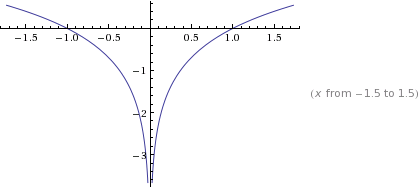
\includegraphics[scale=0.5]{log_x.png}

\subsection{\texorpdfstring{$\frac{1}{x}$}{1/x}}
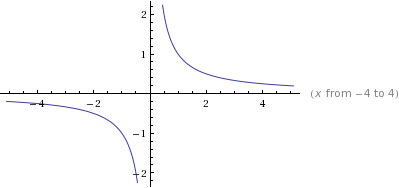
\includegraphics[scale=0.5]{1_over_x.png}

\subsection{\texorpdfstring{$\sqrt{x}$}{x^(1/x)}}
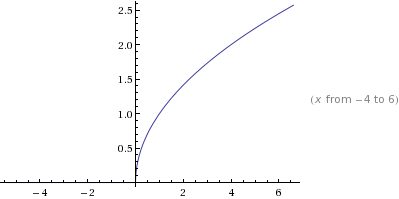
\includegraphics[scale=0.5]{sqrt_x.png}

\subsection{Funktionsmanipulation}
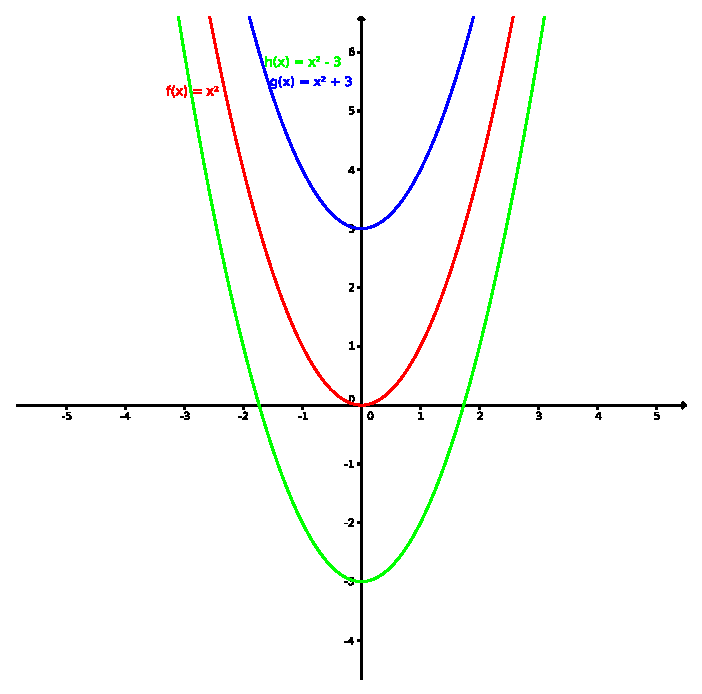
\includegraphics[width=\columnwidth]{manipulation_1.eps}
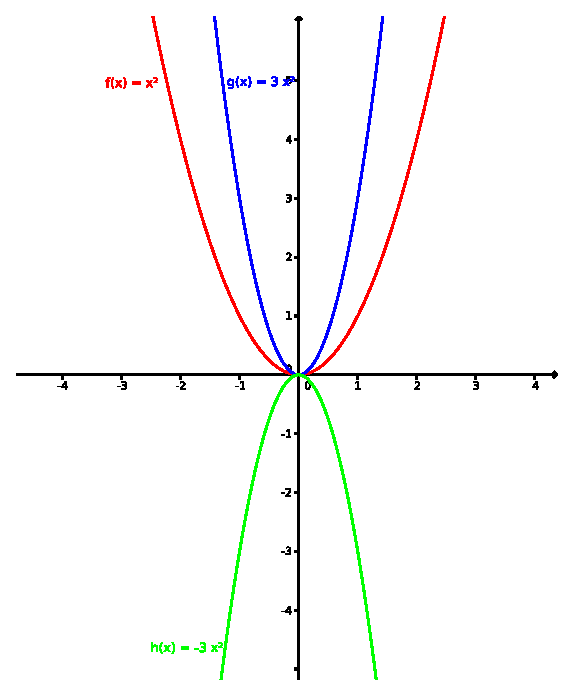
\includegraphics[width=\columnwidth]{manipulation_2.eps}
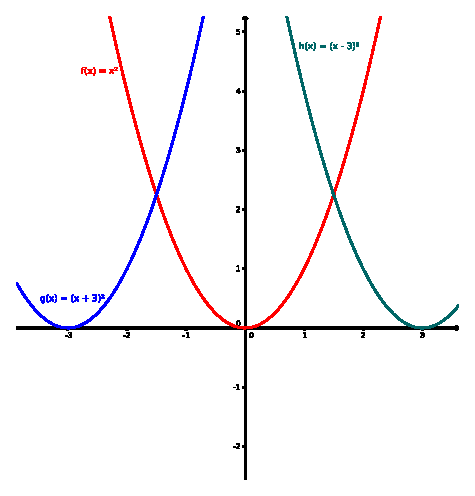
\includegraphics[width=\columnwidth]{manipulation_3.eps}

\subsection{Pascalsches Dreieck}
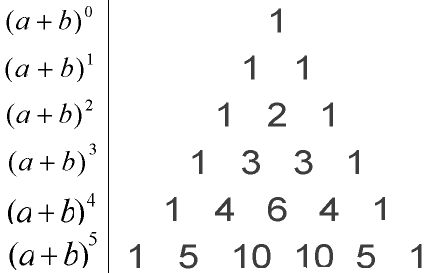
\includegraphics[width=\columnwidth]{pascal.png}

\end{multicols}\end{landscape}


% fill the page
\clearpage

\end{document}
